\section{Аналитический раздел}

\subsection{Введение}
\todo[inline]{Заполнить введение}

\subsection{Понятие ключевого слова}

Первые попытки теоретического решения проблемы выделения ключевых ("опорных", "обобщающих") слов была предпринята в работе А.Н. Соколова Внутренняя речь и мышление \cite{6}.
Основы современного понимания ключевых слов, можно сформулировать следующим образом \cite{7}:
\begin{enumerate}
	\item ключевые слова отображают тему текста;
	\item их упорядоченность в наборе ключевых слов может трактоваться как эксплицитно невыраженная тема текста;
	\item набор ключевых слов рассматривается как один из минимальных вариантов "текста";
	\item такого типа "текст" характеризуется "ядерной" цельностью и минимальной связностью
\end{enumerate}

Ключевые слова - это одно или многокомпонентные лексические группы, отражающие содержание документа \cite{3}

\subsection{Извлечение ключевых слов}

Извлечение ключевых слов (Keyword extraction) - это задача по автоматическому определению набора терминов которые наилучшем образом описывают объект документа.
При изучении терминов, представляющих наиболее релевантную информацию, содержащуюся в документе, используется различная терминология: ключевые фразы, ключевые сегменты, ключевые термины, или просто ключевые слова.
Все выше перечисленные синонимы имеют одну и туже функцию - охарактеризовать обсуждаемую тему в документе \cite{4}.
Извлечение маленького множество элементов представляющих из себя от одного и более терминов из одного документа является важной проблемой в "Информационном поиске" (Information Retrieval, IR), "Интеллектуальном анализе текста" (Text mining, TM) и в "Обработке естественного языка" (Natural Language Processing, NLP).

\todo[inline]{Добавить описание TM, NLP, IR}

Ключевые слова нашли широкое применение в запросах к системам информационного поиска, по сколько их легко определить, пересмотреть, запомнить и поделиться.
По сравнению с математическими сигнатурами, они независимы от любого корпуса и могут применяться в нескольких корпусах и системах ИП \cite{5}
Так же ключевые слова используются для улучшения функциональности Информационно поисковых систем.
Другими словами они могут быть использованы для создания автоматического индекса для коллекции документов или, в качестве альтернативы, могут использовать для представления документов в задачах категоризации или классификации \cite{1}.

Извлечение краткого изложения - это основная задача многих IR и NLP приложений включая в себя автоматическое индексирование, обобщение, управление документами, высокоуровневое семантическое описание, категоризацию или кластеризацию текста, документов или веб-сайтов, поиск по категориям, создание словарей для конкретной области, распознавание имен, определение тем, отслеживание и т.д.
Благодаря тому что назначение ключевых слов документам в ручную является очень дорогостоящей, трудоемкой и утомительной задачей и дополнительно к этому количество доступных цифровых документов растет, автоматическое извлечение ключевых слов привлекло интерес исследователей в последние несколько лет.
Хотя приложения для извлечения ключевых слов обычно работаю с отдельными документами, извлечение так же используется для более сложных задач (Извлечение из коллекции текстов, всего веб-сайта и т.п.)

Общая схема извлечения ключевых слов из текста практически одинакова для всех используемых методов и состоит из следующих шагов:
\begin{enumerate}
	\item предварительная обработка текста:
	\item \begin{enumerate}
		\item исключение элементов маркировки;
		\item приведение слова к словарной форме;
		\item удаление стоп слов, не несущих смысловой нагрузки (предлоги, союзы, частицы, местоимения, междометия и т.д.)
	\end{enumerate}
	\item отбор кандидатов в ключевые слова;
	\item фильтрация кандидатов в ключевые слова (анализ значимых признаков для каждого кандидата)
\end{enumerate}

\subsection{Систематизация методов}

\todo[inline]{Переосмыслить систематизацию методов}

Методы назначения ключевых слов можно условно разделить 2 категории:
\begin{enumerate}
	\item назначение ключевых слов;
	\item извлечение ключевых слов;
\end{enumerate}

Оба они вращаются вокруг одной и той же проблемы - выбора лучшего ключевого слова.
При назначение ключевых слов, оные выбираются из контролируемого словаря терминов или предопределенной таксономии, а документы подразделяются на классы в соответствии с их содержанием.
Извлечение ключевых слов обогащает документ ключевыми словами, которые явно упоминаются в тексте.
Слова, встречающиеся в документе, анализируются с целью выявления наиболее репрезентативных из них, обычно исследую 2 свойства источника (частота и длина).
Обычно извлечение ключевых слов не используется предустановленный словарь для определения ключевых слов.
В данной работе "Назначение ключевых слов" рассматриваться не будет.

Изучив работы \cite{8} методы могут быть разделены на следующие группы:
\begin{enumerate}
	\item статистический подход;
	\item машинное обучение;
\end{enumerate}
Или более детализировано:
\begin{enumerate}
	\item статистический подход;
	\item лингвистический подход;
	\item подход через машинное обучение;
	\item комбинированный;
	\item остальное;
\end{enumerate}

Так же стоит отметить что способы извлечения ключевых слов можно категоризировать на контролируемые (supervized) и неконтролируемые (unsupervized) методы.
Самым распространенным методом из первой категории является KEA (keyphrase extraction algorithm).
Данный метод использует Наивный Байесовский алгоритм для обучения и извлечения ключевых выражений.
Двумя главными проблемами контролируемых методов является обязательное наличие тренировочных данных с в ручную размеченными ключевыми словами и привязанности к доменной области, на которой они обучались \ref{fig:ketypes}.

\missingfigure[figwidth=6cm]{Добавить новое изображение классификации методов}

\begin{figure}[H]
	\centering
	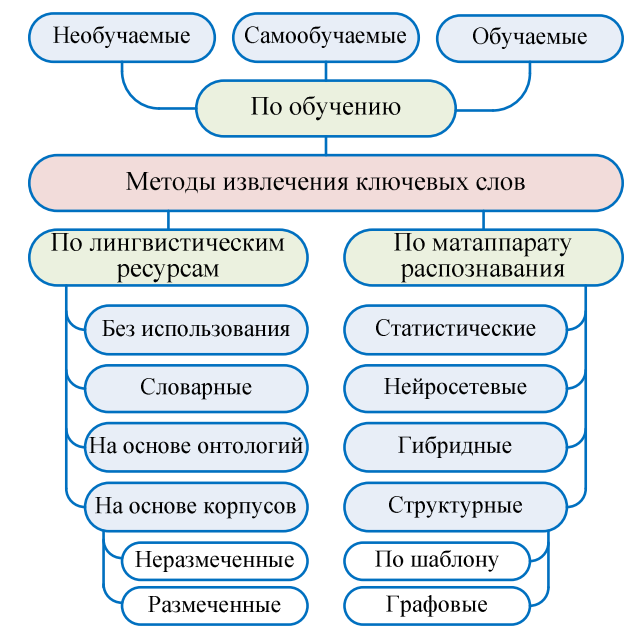
\includegraphics[width=0.7\linewidth]{src/img/ke_types}
	\caption[]{Классификация методов извлечения ключевых слов}
	\label{fig:ketypes}
\end{figure}

\subsubsection{Статистические методы}
Статистические методы извлечения ключевых слов работают на основе численных данных, говорящих о встречаемости слова в тексте.
К статистическим методам относятся:
\begin{enumerate}
	\item TF-IDF;
	\item YAKE;
	\item Rake
\end{enumerate}

\textbf{TF-IDF} - это аббревиатура, скрывающая за собой "Term Frequency - Inverse Document Frequency" (Частота термина и инвертированная частота в документе).

Еще в 1958 году Ганс Петер Лун в своей статье "Автоматическое создание литературных рефератов" предложил, что "частота появления слов в статье обеспечивает полезное измерение значимости слов" что до сих пор, вероятно, является одни из самых важных аспектов в области "Информационного поиска". 
Данный метод используется во всех известных поисковых системах от Goggle и Yahoo и заканчивая специализированными поисковыми решениями, такими как ElasticSearch и ManticoreSearch \cite{12}.
Как можно понять сверху идет речь про TF.

В 1972 Карен Спарк Джонес в работе "A statistical interpretation of term specificity and it's application in retrieval" в журнале "Journal of Documentation" \cite{11} предложил "Полнота описания документа - это количество содержащихся в нем терминов, а специфичность термина - это количество документов к которым он относится". 
В будущем данная работа станет известна как "inverse document frequency" или IDF.

С помощью tf-idf вместо представления термина в документе его необработанной частотой (количество вхождений) или его относительной частотой (количество терминов, деленное на длину документа), каждый термин взвешивается путем деления частоты термина на количество документов, корпусы которых содержат данное слово.

\textbf{Yake} - Yet Another Keyword Extractor.
Данный метод был разработан компанией LIAAD и первое упоминается в работе "YAKE Keyword extraction from single documents using multiple local features" \cite{14}
Это легковесный автоматический подход извлечения ключевых слов, основанный на статистических характеристиках текста, извлеченных из отдельных документов, для выбора наиболее важных ключевых слов текста. 
Авторы данного способа выделяют следующие особенности \cite{14}:
\begin{enumerate}
	\item не требует обучения
	\item не требует корпуса тематически заготовленных текстов;
	\item не зависит от области использования;
	\item не зависит от языка;
	\item масштабируемость;
	\item результат не зависит от частоты термина;
\end{enumerate}

\textbf{RAKE} - Rapid Automatic Keyphrase Extraction.
К особенностям относят \cite{15}:
\begin{enumerate}
	\item не требует обучение;
	\item не зависит от области применения;
	\item не привязан к определенному языку;
	\item работает на одиночном документе
\end{enumerate}
Во время работы над RAKE у авторов стояла задача разработать механизм, метод извлечения ключевых слов, эффективно работающий c отдельными документами, позволяя примение к динамическим коллекциям, легко применимый к новым доменам.

Преимуществами чисто статистического подхода являются универсальность алгоритмов извлечения ключевых слов, простота реализации и отсутствие необходимости в трудоемких и время-затратных процедурах построения лингвистических баз знаний.
Несмотря на указанные преимущества статистических методов извлечения ключевых слов, чисто статистические методы часто не обеспечивают удовлетворительного качества результатов. 
При этом область их применения ограничена языками с бедной морфологией, такими как английский, где частотность словоформ одной лексемы велика. 
Чисто статистические модели извлечения ключевых слов, удовлетворительно работающие, например, на материале английского языка, не пригодны для естественных языков с богатой морфологией, в частности, для русского языка, где каждая лексема характеризуется большим количеством словоформ с низкой частотностью в каждом конкретном тексте \cite{9}.

К статистическим методаи использующие графовые методам относятся:
\begin{enumerate}
	\item Textrank;
	\item SingleRank
	\item ExpandRank
	\item TopicRank;
	\item TopicalPageRank
	\item PositionalRank
	\item MultipartiteRank
	\item Rake;
\end{enumerate}

\subsubsection{Лингвистические}
\subsubsection{Гибридные}
\subsection{Заключение}

